\section*{Transformación y Jacobiano}

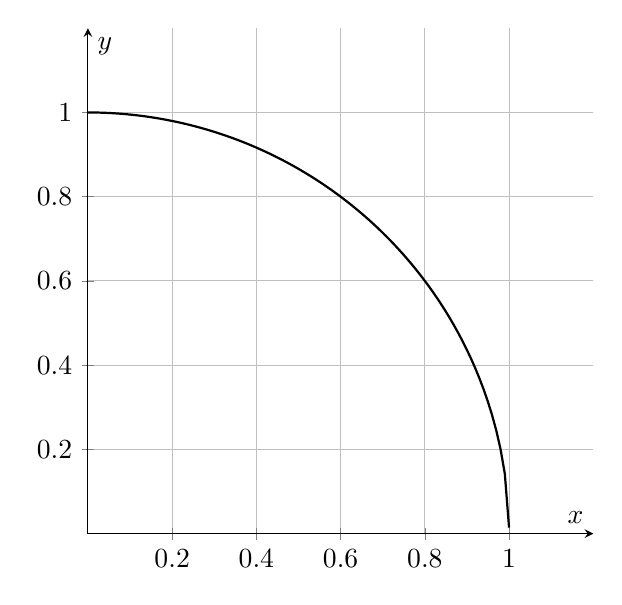
\begin{tikzpicture}
    \begin{axis}[ 
        axis lines=middle,
        xmin=0, xmax=1.2, % Límites en x
        ymin=0, ymax=1.2, % Límites en y
        xtick={0,0.2,0.4,0.6,0.8,1},
        ytick={0,0.2,0.4,0.6,0.8,1},
        xlabel={$x$}, ylabel={$y$},
        grid=both,
        width=8cm, height=8cm
    ]
        % Graficar el cuarto de círculo
        \addplot[
            domain=0:1, 
            samples=100, 
            thick
        ] ({x}, {sqrt(1-x^2)});
    \end{axis}
\end{tikzpicture}

El límite de \( D^* \) está dado por \( u = 0 \), \( v = 0 \), \( u^2 + v^2 = 1 \), con las transformaciones:
\[
x = u^2 - v^2, \quad y = 2uv
\]
Por el Jacobiano directo, tenemos:
\[
\frac{\partial(x,y)}{\partial(u,v)} = \left| \begin{matrix} \frac{\partial x}{\partial u} & \frac{\partial x}{\partial v} \\ \frac{\partial y}{\partial u} & \frac{\partial y}{\partial v} \end{matrix} \right|
\]
Calculando las derivadas parciales:
\[
\frac{\partial x}{\partial u} = 2u, \quad \frac{\partial x}{\partial v} = -2v, \quad \frac{\partial y}{\partial u} = 2v, \quad \frac{\partial y}{\partial v} = 2u
\]
El Jacobiano es:
\[
J = \left| \begin{matrix} 2u & -2v \\ 2v & 2u \end{matrix} \right| = 4u^2 + 4v^2 = 4(u^2 + v^2)
\]
Como la región \( D^* \) está definida por \( D^* = \{(u,v) | u^2 + v^2 \leq 1, u \geq 0, v \geq 0 \} \), el diferencial en \( (x,y) \) es:
\[
dx\,dy = |4(u^2 + v^2)| \, du\,dv = 4(u^2 + v^2) \, du\,dv
\]
La integral sobre la región \( D^* \) en \( (u,v) \) es:
\[
\iint_D dx\,dy = \iint_{D^*} 4(u^2 + v^2) \, du\,dv
\]
Los límites de integración para \( u \) van de 0 a 1, y \( v \) va de 0 a \( \sqrt{1 - u^2} \). Por lo tanto, la integral es:
\[
\int_0^1 4 \int_0^{\sqrt{1-u^2}} (u^2 + v^2) \, dv \, du
\]
La integral en coordenadas cartesianas es:
\[
I = \int_0^1 \int_0^{\sqrt{1-x^2}} 4(x^2 + y^2) \, dy \, dx
\]
Esto corresponde al cuarto de círculo en el primer cuadrante con \(x^2 + y^2 \leq 1\).

\section*{Resolver la integral interior}

La integral interior es:
\[
\int_0^{\sqrt{1-x^2}} 4(x^2 + y^2) \, dy
\]

\[
\int_0^{\sqrt{1-x^2}} 4(x^2 + y^2) \, dy = 4 \int_0^{\sqrt{1-x^2}} x^2 \, dy + 4 \int_0^{\sqrt{1-x^2}} y^2 \, dy
\]

\subsection*{Primera parte: \( 4 \int_0^{\sqrt{1-x^2}} x^2 \, dy \)}

Dado que \(x^2\) es constante respecto a \(y\), esta integral es:
\[
4 \int_0^{\sqrt{1-x^2}} x^2 \, dy = 4 x^2 \left[ y \right]_0^{\sqrt{1-x^2}} = 4 x^2 (\sqrt{1 - x^2})
\]

\subsection*{Segunda parte: \( 4 \int_0^{\sqrt{1-x^2}} y^2 \, dy \)}

La integral de \(y^2\) con respecto a \(y\) es:
\[
4 \int_0^{\sqrt{1-x^2}} y^2 \, dy = 4 \left[ \frac{y^3}{3} \right]_0^{\sqrt{1-x^2}} = 4 \cdot \frac{1}{3} \left( (1 - x^2)^{3/2} \right)
\]

Entonces:
\[
\int_0^{\sqrt{1-x^2}} 4(x^2 + y^2) \, dy = 4 x^2 (\sqrt{1 - x^2}) + \frac{4}{3} (1 - x^2)^{3/2}
\]

\section*{Resolver la integral exterior}

Con respecto a \(x\), la integral es:
\[
I = \int_0^1 \left[ 4 x^2 (\sqrt{1 - x^2}) + \frac{4}{3} (1 - x^2)^{3/2} \right] dx
\]
Dividiendo en dos integrales separadas:
\[
I = \int_0^1 4 x^2 (\sqrt{1 - x^2}) \, dx + \int_0^1 \frac{4}{3} (1 - x^2)^{3/2} \, dx
\]

\subsection*{Primera integral: \( 4 x^2 (\sqrt{1 - x^2}) \)}

Usamos el cambio de variable \( u = 1 - x^2 \), con \( du = -2x \, dx \). Los límites cambian:
- Cuando \( x = 0 \), \( u = 1 \)
- Cuando \( x = 1 \), \( u = 0 \)

\[
\int_0^1 4 x^2 (\sqrt{1 - x^2}) \, dx = \int_1^0 4 u^{1/2} \left( -\frac{1}{2} du \right) = \int_0^1 2 u^{1/2} \, du
\]

\[
\int_0^1 2 u^{1/2} \, du = 2 \cdot \frac{2}{3} u^{3/2} \bigg|_0^1 = \frac{4}{3}
\]

\subsection*{Segunda integral: \( \frac{4}{3} (1 - x^2)^{3/2} \)}

Usamos el mismo cambio de variable \( u = 1 - x^2 \):
\[
\int_0^1 \frac{4}{3} (1 - x^2)^{3/2} \, dx = \frac{4}{3} \int_1^0 u^{3/2} \left( -\frac{1}{2} du \right) = \frac{2}{3} \int_0^1 u^{3/2} \, du
\]

Resolviendo:
\[
\frac{2}{3} \int_0^1 u^{3/2} \, du = \frac{2}{3} \cdot \frac{2}{5} u^{5/2} \bigg|_0^1 = \frac{4}{15}
\]

\section*{Resultado}

Sumando ambas integrales:
\[
I = \frac{4}{3} + \frac{4}{15} = \frac{20}{15} + \frac{4}{15} = \frac{24}{15} = \frac{8}{5}
\]

\newpage  % Esto agrega un salto de página

\section*{Cálculo de la Integral con Coordenadas Polares}

La integral es:
\[
\int_0^1 4 \int_0^{\sqrt{1-u^2}} (u^2 + v^2) \, dv \, du
\]
Puede resolverse usando coordenadas polares, donde las transformaciones son:
\[
u = r \cos \theta, \quad v = r \sin \theta
\]
Aquí, \(r\) es el radio y \(\theta\) es el ángulo. Dado que estamos trabajando en el primer cuadrante, tenemos:
\[
r \text{ va de } 0 \text{ a } 1, \quad \theta \text{ va de } 0 \text{ a } \frac{\pi}{2}
\]
La integral en coordenadas polares se convierte en:
\[
\iint_D 4(u^2 + v^2) \, du \, dv = \int_0^{\frac{\pi}{2}} \int_0^1 4r^2 \cdot r \, dr \, d\theta
\]
Ahora, calculamos el Jacobiano de la transformación:
\[
\frac{\partial(x,y)}{\partial(r,\theta)} = \left| \begin{matrix} \frac{\partial x}{\partial r} & \frac{\partial x}{\partial \theta} \\ \frac{\partial y}{\partial r} & \frac{\partial y}{\partial \theta} \end{matrix} \right| = \left| \begin{matrix} \cos \theta & -r \sin \theta \\ \sin \theta & r \cos \theta \end{matrix} \right| = r(\cos^2 \theta + \sin^2 \theta) = r
\]
Por lo tanto, la integral se convierte en:
\[
\int_0^{\frac{\pi}{2}} \int_0^1 4r^3 \, dr \, d\theta
\]
Separando las integrales:
\[
\int_0^{\frac{\pi}{2}} d\theta \left( \int_0^1 4r^3 \, dr \right)
\]
\[
\int_0^1 4r^3 \, dr = \left[ \frac{4r^4}{4} \right]_0^1 = \left[ r^4 \right]_0^1 = 1^4 - 0 = 1
\]
\[
\int_0^{\frac{\pi}{2}} d\theta = \frac{\pi}{2}
\]
Por lo tanto, al multiplicar las integrales:
\[
\frac{\pi}{2}
\]
